\chapter{4.Fejlesztés}

A technológiák kiválasztása után, de még a web áruház lefejlesztése előtt a következő lépés az oldal kinézetének megtervezés. A web áruházamat úgy képzeltem el, amely képes nagy mennyiségű termék megjelenítésére és képes e termékek tárolására adatbázisban.  Az oldal megtervezésénél oda kell figyelni, hogy fel legyen szerelve egy egyszerűbb keresővel és szűrési lehetőségekkel, hogy a jövőbeli felhasználók számára könnyen kezelhető legyen. Olyan oldalt akartam volna létrehozni, amelyet a jövőbeli felhasználók előszeretettel fognak használni a későbbiekben.

\section{Oldalak megtervezése}

Két féle típusú oldalt terveztem meg. Az első azok az oldalaknak a csoportja, amelyeket azok a felhasználók láthatnak, amelyek még nem jelentkeztek be az oldalra. Ebbe a csoportba soroltam be azokat az oldalakat, amely fogadja a felhasználót az oldal meglátogatásakor, továbbá a bejelentkező, regisztrációs oldal, termékek általános megtekintését és a kosár ahol megnézheti a felhasználó a vásárolni kívánt termékeket. A második csoport azokat az oldalakat tartalmazza, amelyeket a felhasználók és a regisztráció és a bejelentkezés után láthatnak, ilyen oldalak a pénztár és a fizetés, amelyeket csak a bejelentkezés után tekinthet meg a felhasználó.

Az egyszerűbb kezelhetőségek miatt az oldalt komponensekre osztottam fel azon belül is oldalakra (pages) és részlegekre (partials). A részlegekre azért volt szükség, mert némely oldalakat több komponensből állítottam össze. Ezekre a kód egyszerűsítése miatt volt szükség vagy, éppen azért mert némely részleget több oldalon is felhasználtam.\\

A komponensek ez alapján:\\

\textbf{Pages}
\begin{itemize}
    \item Cart – ez a kosár ez tartalmazza azokat a termékeket, amelyeket a vásárló meg szeretne venni.
    \item Checkout – Ezen az oldalon tekintheti meg a felhasználó a megvásárolni kívánt termékek és áruk összesítését. További itt található a megrendelési űrlap és egy térkép a szállítás helyének kiválasztásához.
    \item Coin – ezen az oldalon láthatják nagyban a termékeket
    \item Home – ez az alap oldal ahol az összes termék fel van sorolva
    \item Login – ez a bejelentkezési oldal
    \item Payment – ez hasonló a checkout-hoz de ez után már a fizetés jön
    \item Register –ez a regisztrációs oldal
\end{itemize}

\textbf{Partials}
\begin{itemize}
    \item default-button – az alap gombok komponense
    \item header – az oldalak fejléce
    \item input-container – a login register és a checkout komponenseknél a beviteli mezők összegzésehez
    \item input-validation – a beviteli mezők ellenőrzéséhez használtam
    \item loading – töltő képernyő
    \item map – térkép a checkout-hoz
    \item not-found – gomb a főoldalra való visszatéréshez
    \item order-items-list – rendelt termékek listája
    \item search - kereséshez
    \item star-rating – a termék ritkaságának a jelöléséhez
    \item tags – szűréshez
    \item text-input – beviteli mezők
    \item title – címek
\end{itemize}

\section{Oldalak leírása}
A home oldal megtervezésénél és elkészítésénél egy olyan oldalt akartam létrehozni, amelyre a jövőbeli felhasználók szívesen visszatérnek. Ezt próbáltam megoldani egy minimalista stílussal. Az oldal látható a kereső, amelyben kereshetünk az adott termékek után. Ez alatt a különféle termékekre szűrhetünk különböző címkék alapján attól függően, hogy az adott termékeknek milyen tulajdonságaik vannak. Továbbá a címkék alatt kis kártyák láthatóak ahol a termékek láthatóak. Minden kis kártyán, helyett kapott a termékről egy kép, a termék neve és mellette egy szívecske, amely azt jelzi, hogy az adott terméket mennyire kedvence a vásárlóknak. Továbbá a kártya tartalmazz egy csillag rendszert, amely azt mutatja, hogy a termék mennyire ritka. Ez alatt foglal helyet a termék tulajdonságai és ára forintban megadva.

\begin{figure}[h]
\centering
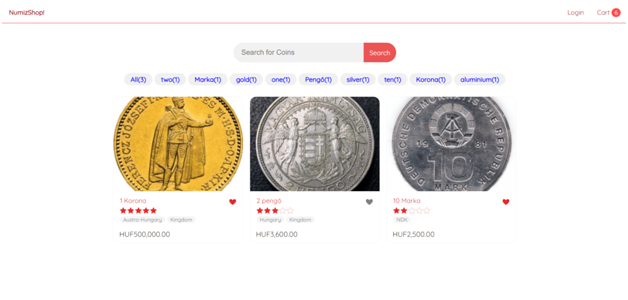
\includegraphics[scale=1]{images/home.png}
\caption{A főoldal megjelenítése.}
\label{fig:fo_oldal}
\end{figure}

Minden oldal tetején látható a fejléc sáv. Az oldal logójára kattintva mindig a fő oldalra fog vezényelni. A jobb felső sarokban a login gombra kattintva a bejelentkező oldalra vezérel át ahol képesek vagyunk belépni vagy ha még nincs felhasználói fiókunk onnan tudunk átnavigálni a regisztrációs oldalra. A login gomb mellett található a cart gomb, amely tovább navigál a kosárhoz. Ezen a gombon folyamatosan láthatjuk, hogy mennyi terméket helyeztünk a kosárba. Ez a kis funkciót azért raktam bele az oldalba, hogy a vásárlóknak még kényelmesebb legyen az oldal használat így nincs szükségük belépni a kosárba, hogy tudják, hogy mennyi termékük van már. A login oldal egyszerűen van felépítve csak középen a belépő űrlap és alatta egy gomb, ha a regisztrációs oldalra akar átnavigálni az ember. A register oldal is így van, felépítve csak itt regisztrációs űrlap van és a gomb a login oldalra vezényel át. A coin oldal akkor jelenik, meg amikor a fő oldalon rákattintunk valamelyik termék kártyájára. Ez további információkat tartalmaz a termékről, mint például a pontos névértéke, az anyaga és a pontos neve. Ezen felül nagyobb méretben láthatjuk az adott terméket.

A cart oldalra átnavigálva láthatjuk a kosarunk tartalmát. Itt a megvásárolni kívánt termékek felvannak sorolva egymás alatt kis léceken. Ezeken a léceken állíthatjuk hogy az adott termékből mennyit szeretnénk vásárolni és hogy nagyobb mennyiségben mennyibe fog kerülni. Viszont arra az esetre is gondolni kell ha a vásárló csak félre kattintott így egy törlés gombot is elhelyeztem amivel az adott terméket eltávolíthatjuk a kosárból. A lécek mellett egy összeítő fült hoztam létre amely tartalmazza a termékek össz árát és ártéket ez alatt pedig egy gomb amely a pénztárhoz vezet tovább. Viszont a pénztárhoz csak bejelentkezés után lehet navigálni. Ezért ha regisztráció nélkül nyomunk a gombra akkor a bejelentkezési oldalra fog navigálni.

\begin{figure}[h]
\centering
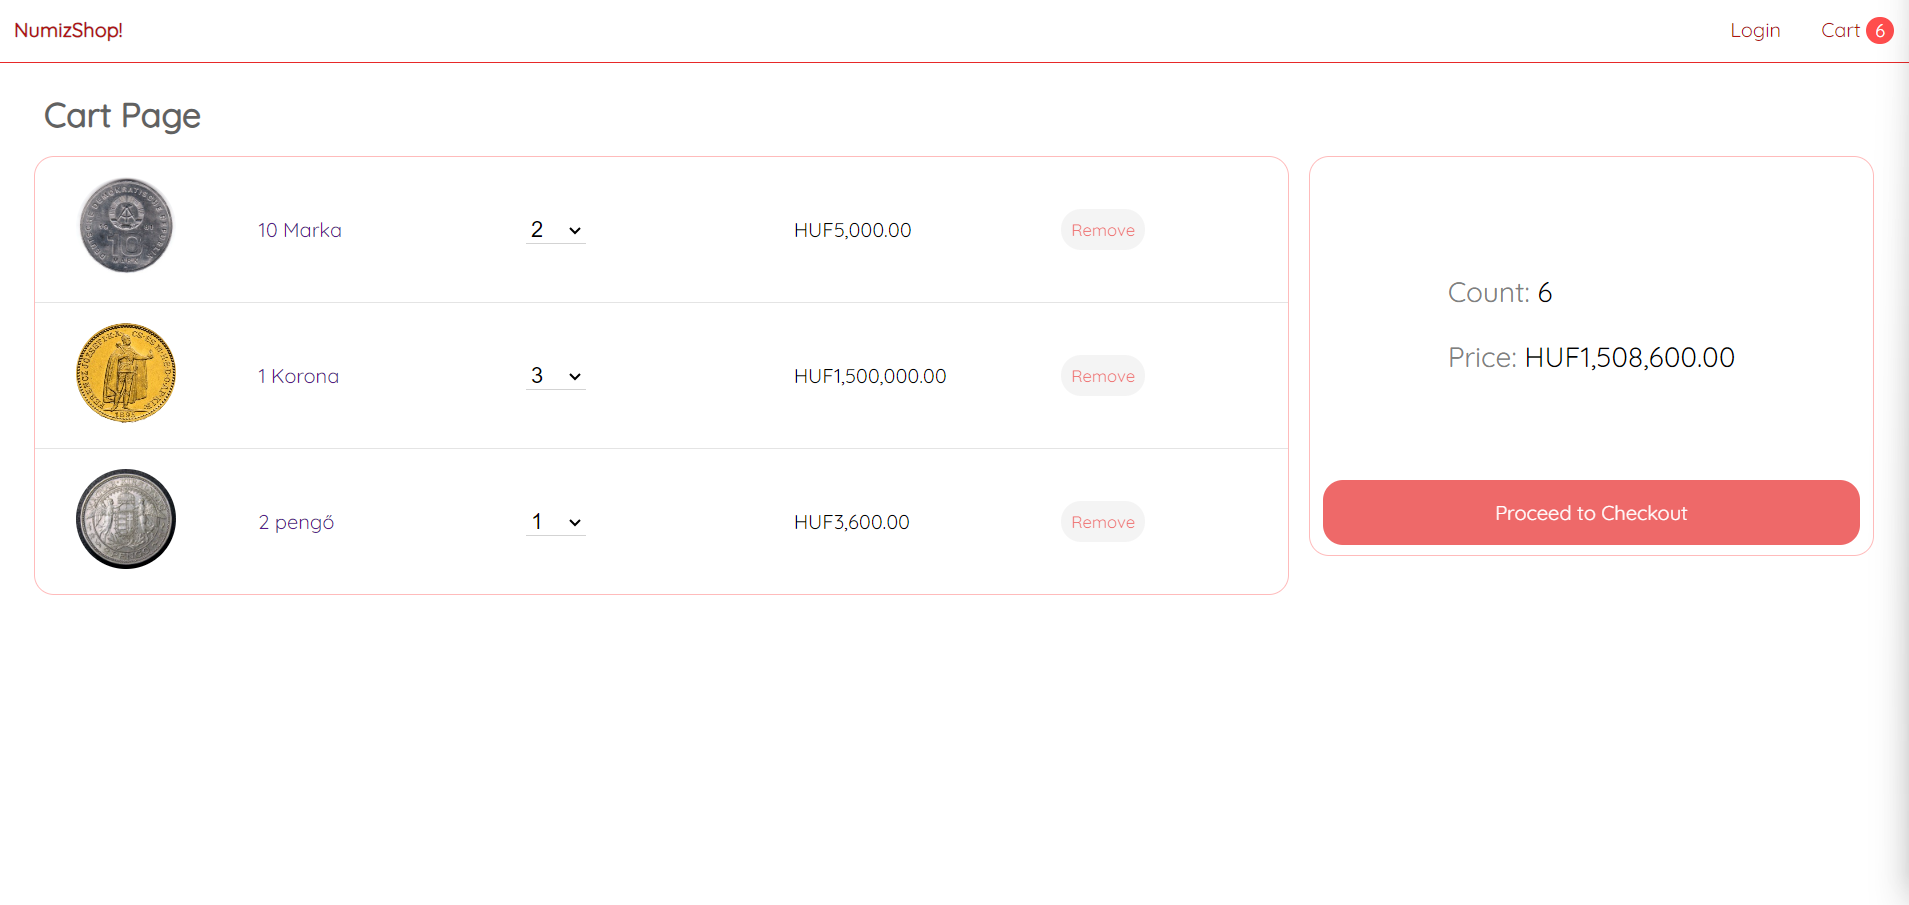
\includegraphics[scale=0.3]{images/cart.png}
\caption{A kosár megjelenítése a webáruházban.}
\label{fig:kosar}
\end{figure}

Ha már viszont be vagyunk jelentkezve és tovább navigálunk a pénztár oldalra. Akkor itt is láthatjuk a megvásárolni kívánt termékeket azok össz és darab értékét, és hogy melyik termékből mennyit akarunk vásárolni hasonlóan a kosár oldalához. Továbbá meg kell adnunk a vevő nevét és lakcímét. Ezek mellett található egy világtérkép, amivel a pontos helyzetünket adhatjuk meg a szállítás megkönnyítéséhez. A térképen található egy gomb, amellyel rögtön a saját helyzetünkhöz ugrik a térkép ezzel a felhasználó dolgát megkönnyítve a kellemesebb használat érdekében. A térkép létrehozásához egy külön komponenst azon belül is egy részleget hoztam létre ezt annak az érdekében, hogy a kód átláthatóbb legyen mivel több beállítást is véghez kellett vinni a térképen.

\begin{figure}[h]
\centering
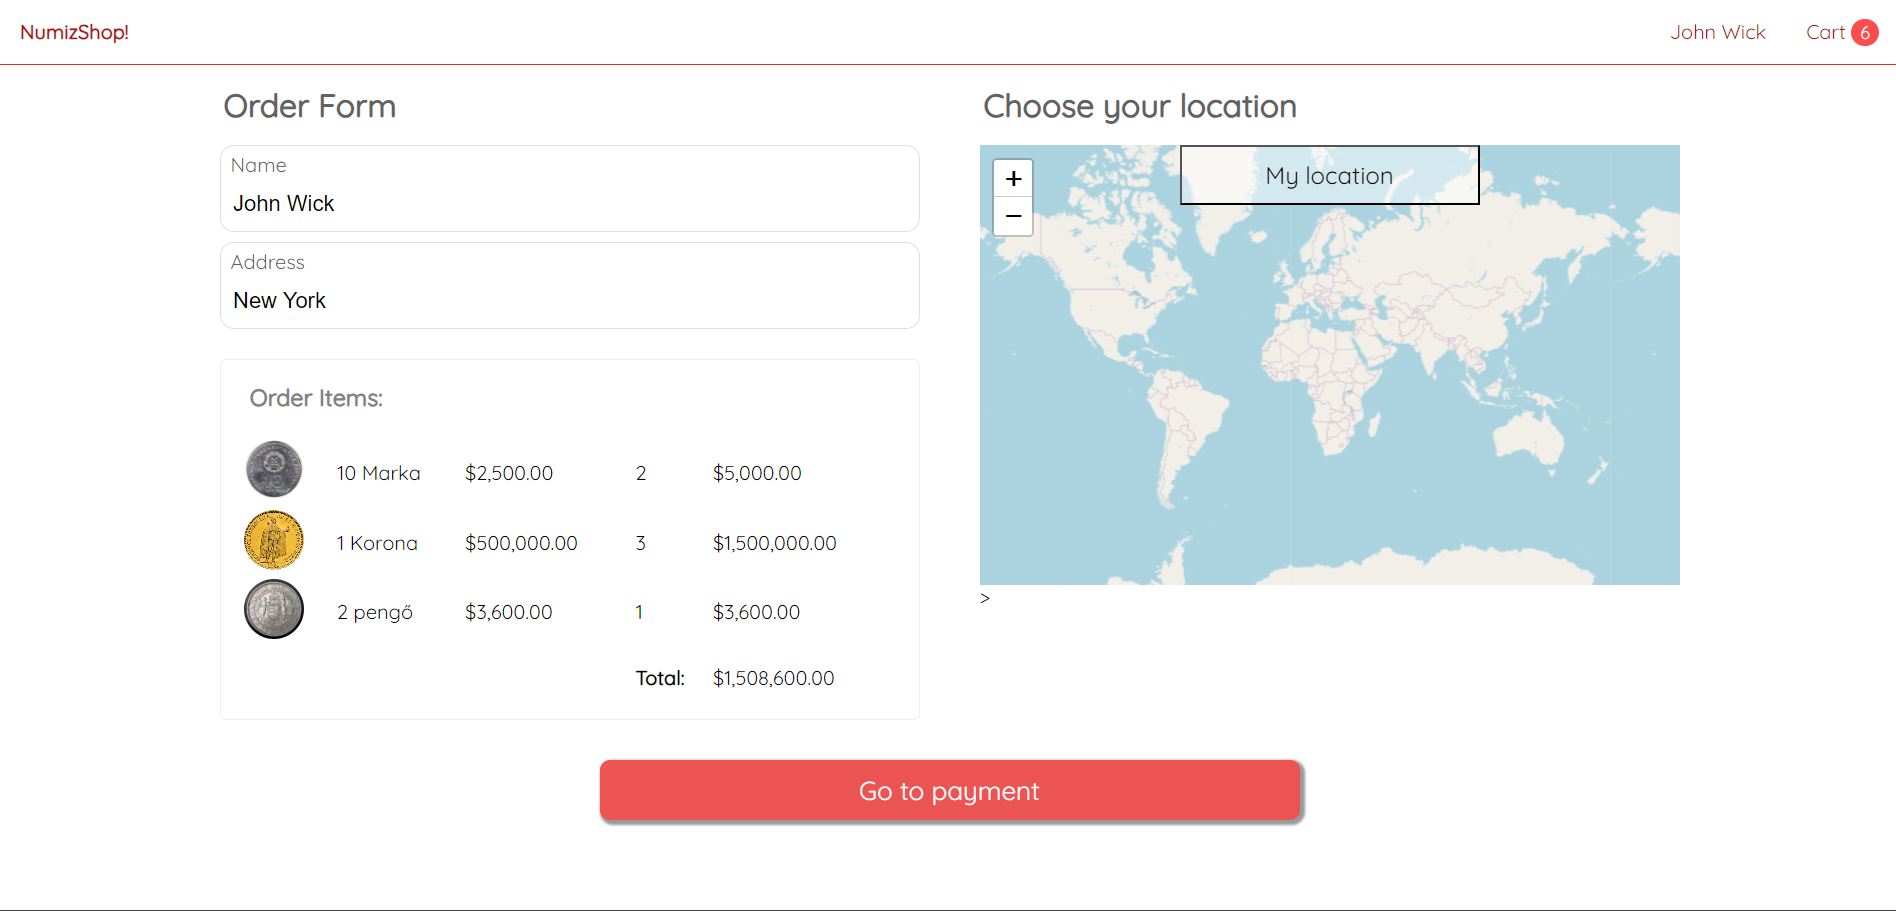
\includegraphics[scale=0.3]{images/checkout.png}
\caption{A pénztár megjelenítése a webáruházban.}
\label{fig:penztar}
\end{figure}

Ha a pénztár oldal alján tovább navigálunk payment (fizetés) oldalra ugyan az az oldal fog fogadni, mint a pénztár oldalán viszont itt már az oldal alján egy paypal vagy más egyébb fizetési mód fogadja a felhasználót ez a része viszont nincs lefejlesztve, de erre a jövőbeli terveknél majd visszatérek. Azokban a pillanatokban, amikor két oldal között navigálunk, és az oldal tölt arra az esetre létrehoztam egy komponenst, amely a töltőképernyőt biztosítja ez a partials mappában a loading az itt található töltő képet a loading.io [hivatkozás] oldal segítségével hoztam létre saját magam. A jövőbeli felhasználók segítségére létrehoztam még egy fontos komponenst a partials mappába az input-validation-t.

\begin{figure}[h]
\centering
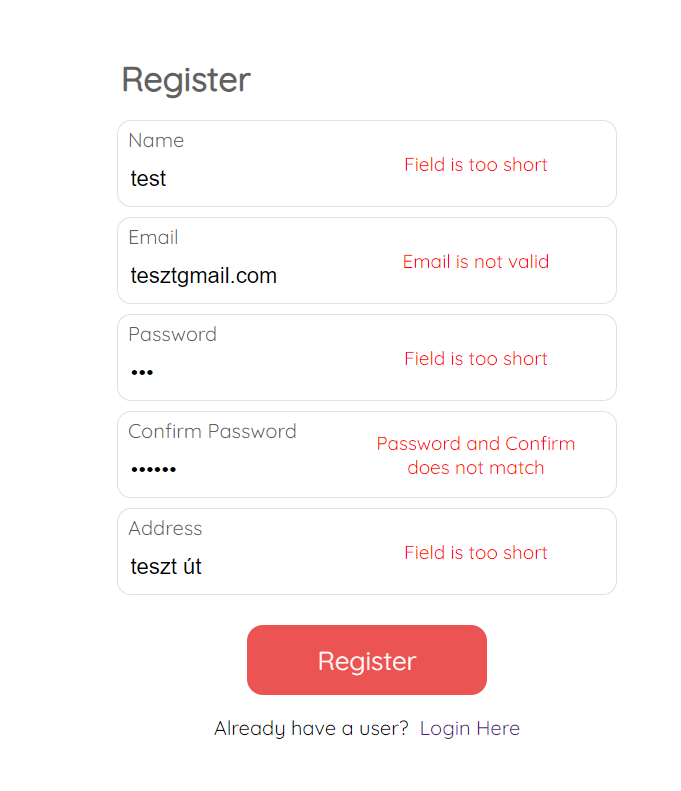
\includegraphics[scale=0.6]{images/validation.png}
\caption{A beviteli mezők validálása.}
\label{fig:validacio}
\end{figure}

Ezt akkor használom, amikor regisztrálnánk vagy bejelentkeznénk. Ez a komponens ellenőrzi azt, hogy a beviteli mezőkben érvényes adatokat adjanak meg a felhasználók. Regisztrációnál szól, ha túl rövid nevet vagy jelszót ad meg a felhasználó vagy például nem megfelelő formátumú az email cím. Ez a komponens is azért hoztam létre ami az egyik fő célom is volt hogy egy olyan webáruházat hozzak létre amelyet a felhasználók könnyedén kezelni tudnak és baráti a kezelő felülete ami arra sarkalja őket hogy vissza térjenek később is ide.

\subsection{Adatbázis}
Miután már nagyjából összeállt a fejemben hogy hogyan is szeretném, hogy kinézzen a webáruházam frontend része. A következő rész az adatbázis megtervezése volt. Ennek a résznek a megtervezése az egyik legfontosabb feladat, mert ennek függvényében változhat a későbbiekben a frontend kinézete. Meg a program írása közben már pontosan tudtam, hogy milyen adatokkal is kell dolgoznom. Adatbázisnak az áruházhoz a MongoDB-t választottam ezen belül is a MongoDB Atlast. Két verziója van a MongoDB-nek az egy a Compass amely egy letölthető verzió a másik az Atlas amely pedig felhő alapú. Én azért az Atlas mellett döntöttem, mert számomra egyszerűbben használható volt.

Amikor terveztem a frontendet hat darab modell-t hoztam létre ezekből. Ezek közül háromra van biztosan szükségünk meg egyre még szükségünk lehet ha szűrni akarunk az adatbázisban. A három fő modell a Coins, a User és az Order. A szűrő modell pedig a Tag.\\

Ezek a modellek a következő attribútumokat tartalmazzák:

Coins:
\begin{itemize}
    \item id – az érme egyedi azonosítója
    \item name – az érme neve
    \item price – az érme ára
    \item tags – az érme tulajdonságai
    \item favorite – ez mutatja, hogy az érme a kedvencek között van -e
    \item stars – ez mutatja az adott érme ritkaságát
    \item imageUrl – az érméről kép
    \item origins – az érme eredete
\end{itemize}

User:
\begin{itemize}
    \item id – a felhasználó egyedi azonosítója
    \item email – a felhasználó saját email címét tartalmazza, egy email címet csak egyszer lehet használni mivel az oldalra való belépés során a felhasználónak az email címét és jelszavát kell megadnia
    \item name – a felhasználó neve 5 karakternél hosszabbnak kell lenni a regisztrációs validációk miatt
    \item address – a felhasználó címét tartalmazza
    \item token - a felhasználóhoz tartozó tokent tartalmazza
    \item isAdmin – azt tartalmazza, hogy az adott felhasználó az oldalon milyen pozíciót tölt be
\end{itemize}

Order:
\begin{itemize}
    \item id – az érméknek egyedi azonosítója van, amelyeket a cart modell-be helyezünk
    \item items – ez tartalmazza a termék árát és darab számát 
    \item totalPrice – ez tartalmazza a kosár tartalmának teljes összegét
    \item name – ez tartalmazza a vásárló nevét
    \item address – ez tartalmazza a vásárló címét
    \item addressLatLng – ez tartalmazza a vásárló címét, amelyet a térképpel adott meg
    \item paymentId – ez tartalmazza a fizetés egyedi azonosítóját
    \item createdAt – ez tartalmazza, hogy mikor keletkezet a rendelés
    \item status – ez tartalmazza a rendelés állapotát
\end{itemize}

Ezek mellett a kisebb modellek igazából csak a nagyobb modellek kiszolgálására hoztam létre ilyen modell a CartItem amely az Order modell items attribútumát adja. Mint már fentebb említettem a szűrésekhez a Tag modellt használom, melynek csak két attribútuma van a name és a count ennek segítségével tudok az érmék között szűrést végre hajtani.

\subsection{Alap adatok feltöltése}
Az oldal teszteléséhez szükségem volt alap adatokra, ezért a coun.router.ts-be és a user.router.ts-be létrehoztam egy-egy útvűlasztó(router) endpointot amely a /seed útvonalon elérhető. Ezek a végpontok (endpoint) egy aszinkron funkciót hajtanak végre, amely, amelyek az adatbázisba adatokat helyeznek el, ezt angolul seed-nek nevezzük. Az adatokat csak abban az esetben helyezi el az adatbázisban, hogy ha még nincsenek az adatbázisban. A kód pontos működése: a router.get ”/seed” útvonalra érkező GET kéréseket kezel. Ehhez segítséget nyújt az asyncHandler függvény amely megkönnyíti az aszinkron kódblokkok kezelését. Az async (req, res) => aszinkron funkció végrehajtódik amikor a útvonalon való kérés megtörténik a req tartalmazza az érkező kérés adatait, a res-sel pedig választ küldhetünk vissza a kliensnek. Ez után megszámolja az adatbázisban tárolt CoinModel dokumentumainak számát aszinkron módon. Ehhez az ”await”-et használtam, hogy a végrehajtás megálljon, amíg a számlálás folyik. A számolás után ellenőrzöm hogy van-e már adat az adatbázisban. Abban az esetben, ha már van, küld egy választ a kliensnek a ”Seed is already done!” Üzenettel majd a funkció befejeződik. Ha viszont még nincs adat az adatbázisban, akkor a CoinModell alapján létrehoz egy vagy több dokumentumot az adatbázisban. Ezeket az adatokat a ’sample\_coins’ tömbből veszi, majd minden elemhez egy ’id’ tulajdonságot hozzáad, melynek értéke: null. Az ”await”-et ismét használva várakozni fog még az adatbázisba való feltöltés befejeződik. Majd a res.send segítségével választ küld a kliensnek hogy ”Seed is done” tehát a feltöltés (seedelés) folyamat sikeresen megtörtént.

\begin{python}[caption={Alap adatok feltöltése},captionpos=b]
  router.get("/seed", asyncHandler(
  async (req, res) => {
     const usersCount = await UserModel.countDocuments();
     if(usersCount> 0){
       res.send("Seed is already done!");
       return;
     }
 
     await UserModel.create(sample_users);
     res.send("Seed Is Done!");
 }
 ))
\end{python}

\section{Azonosítás megoldása}
Miután megterveztem az adatbázist és a weboldal frontend részét a következő lépés maga a webáruház létrehozása. Mivel egy ilyen jellegű weboldalt remélhetőleg nagy mennyiségű felhasználó fogja látogatni és vásárlásra használni. Ezért fontos szempont volt az elkészítés során a biztonság. Hogy biztosítsam a felhasználók adatait. Szerencsére erre több módszer is létezik. A következőkben az általam használt módokat fogom bemutatni.

Mivel az oldalon való vásárláshoz, regisztrációhoz van szükség ezért a regisztráció és bejelentkező részt írtam meg először. Ugyan is itt van a legnagyobb szükség a biztonságra. A regisztráció folyamán miután a frontend megkapta az adatokat először validálni fogja azt, hogy megfelelnek a megadott jellemzőknek ilyen például, hogy öt karakternél hosszabb név kell, tíz karakternél hosszabb cím, vagy ami segít a felhasználónak, hogy biztosan jó jelszót adjon, meg hogy egyszer ismételten meg kell adnia a jövőbeli jelszavát. Abban az esetben, ha van azonos email cím akkor az oldal szólni fog hogy már regisztrált. Ezek mellet ellenőrzi, hogy a megadott email cím létezik-e már mivel egy email címet csak egyszer lehet használni mivel az oldalra való belépés során a felhasználónak az email címét és jelszavát kell megadnia. Amennyiben sikeres a regisztráció a jelszót hash-elni fogja és tovább küldi az adatbázisnak. 

\subsection{Jelszó titkosítás}
A jelszó védelmére az egyik legalapvetőbb módszer a hashelés ezért választottam én is ezt a módszert. Viszont hozzá kell tenni, hogy ez nem a legbiztonságosabb módszer mivel, vannak olyanok, akik ennek gyengeségeit már ki tudják használni. A működési elve a következő: Kap egy betűkből és számokból álló kombinációt, ezt az algoritmus átalakítja hexadecimális formába bár ez a hash algoritmustól is függ. Előnye hogy bármilyen hosszúságú lehet a jelszó (betűk és számok kombinációja)

\newpage

\begin{python}[caption={Regisztráció},captionpos=b]
  router.post('/register', asyncHandler(
  async (req, res) => {
    const {name, email, password, address} = req.body;
    const user = await UserModel.findOne({email});
    if(user){
      res.status(HTTP_BAD_REQUEST)
      .send('User is already exist, please login!');
      return;
    }

    const encryptedPassword = await bcrypt.hash(password, 10);

    const newUser:User = {
      id:'',
      name,
      email: email.toLowerCase(),
      password: encryptedPassword,
      address,
      isAdmin: false
    }

    const dbUser = await UserModel.create(newUser);
    res.send(generateTokenReponse(dbUser));
  }
))
\end{python}

A bejelentkezés során a jelszót szintúgy hash-elem és így hasonlítom össze a már adatbázisban lévővel. Fentebb már említettem, hogy a hash nem a legbiztonságosabb fajta módszer ezért bcrypt hashelést használtam. Amely saltingot használ az úgy nevezet rainbow table támadások ellen. Mivel a hash hossza mindig azonos és a hashelni kívánt karakter sorozat hossza is minden esetben azonos ezt használja ki a rainbow table támadás is. A jelszavak védelmére ezért kitalálták a saltingot. Itt a jelszó mellé random adatokat rak a bcrypt ezzel védelmet nyújtva a támadások ellen.

\newpage

\begin{python}[caption={Bejelentkezés},captionpos=b]
  router.post("/login", asyncHandler(
  async (req, res) => {
    const {email, password} = req.body;
    const user = await UserModel.findOne({email});
  
     if(user && (await bcrypt.compare(password,user.password))) {
      res.send(generateTokenReponse(user));
     }
     else{
       res.status(HTTP_BAD_REQUEST)
       .send("Username or password is invalid!");
     }
  
  }
))
\end{python}

\subsection{Web Token és Interceptor}
Az adatok biztonsága még így se garantált ezért a sikeres bejelentkezés során generáltatok egy JSON web tokent. Viszont a JSON web token generálása során oda kell figyelni, hogy fontosabb adatokat nem szabad beletenni, mint például bankkártya adatokat vagy hasonló dolgokat.
A generálását én adtam meg az adatok segítségével az alábbi négy részt generálom bele.

\begin{itemize}
    \item User ID -  ezzel lehet azonosítani a, belépet felhasználót
    \item User email – a felhasználó email címe
    \item User isAdmin ebből tudjuk, meg hogy az adott felhasználó milyen pozíciót tölt be az oldalon
    \item JWT\_SECRET ez lesz a titkos kód
\end{itemize}

Az én esetemben ebből a négy dologból fog létrejönni a token. Sikeres bejelentkezés esetén a szerver visszaküldi a tokent és ezt local storage-ban fogja tárolni. Viszont ez így még nem teljesen biztonságos ezért http Interceptort kell használnunk, amely a HTTP request és handler használatával fogja kezelni a beérkező kéréseket. Erre azért van szükség a local storage-t a fejlesztői eszközökkel adatot vihetünk a local storage-ba és már benne lévőket akár felül is írhatjuk.

Az interceptor működése az alábbi: Sikeres bejelentkezés után a már feltöltött tokent lekérdezi abban az esetben, ha a local storage tartalmazza azt akkor leklónozza és a headerben token-ként tárolni fogja azt. Ez után a headerből leklónozott tokent és a szerveren tárolt JWT\_SECRET titkos kódunkat összehasonlítja.

\begin{python}[caption={Interceptor},captionpos=b]
    intercept(request: HttpRequest<unknown>,
    next: HttpHandler): Observable<HttpEvent<unknown>> {
    const user = this.userService.currentUser;
    if(user.token)
    {
      request = request.clone({
        setHeaders:{
          access_token: user.token
        }
      })
    }
    return next.handle(request);
  }
\end{python}

\subsection{Middleware Authorization}
Mivel a főbb funkciókat az oldalon csak akkor lehet használni, ha a felhasználó be van jelentkezve és ezekhez a műveletekhez a oldalnak szüksége van az adott felhasználó id-ra. Ez okból az eddigi védelmek még nem voltak elegendőek még foglalkoznunk kell azokkal a felhasználókkal is, akik úgy próbálják elérni az oldal korlátozott részeit, hogy nem lépnek be. Ez pont azért fontos, mert ha úgy lépne be valaki az oldal e részeire, hogy nincs felhasználói id-je akkor számára ezek a funkciók nem fognak működni. Ezen probléma megoldásásra middleware authorizationt használok. Ez egy olyan szűrő, amely kérések feldolgozása előtt vagy után ellenőrzi, hogy a felhasználó jogosult-e az adott művelet végrehajtására. Ez a szűrő általában az alkalmazás biztonsági rétegét erősíti meg, és megkönnyíti a fejlesztők számára az engedélyek és az autentikáció kezelését. Jelen esetben feladata a fejlécből lekérdezi a token majd ellenőrzi, hogy a token létezik-e, és ha nem a választ elküldi a HTTP\_UNAUTHORIZED státusszal tehát nem rendelkezik a megfelelő jogosultságokkal. A JSON web token-t ellenőrzi a verify függvénnyel amennyiben sikeres hozzá a req.user változóhoz. Azonban ha a JSON Web Token ellenőrzése sikertelen (például lejárt vagy érvénytelen) akkor szintén http\_UNAUTHORIZED státuszt küld vissza. Csak ez után hívja meg a middleware a next függvény, hogy továbbítsa a vezérlést a végpontoknak.

\begin{python}[caption={Middleware Authorization},captionpos=b]
import { verify } from "jsonwebtoken";
import { HTTP_UNAUTHORIZED } from "../constants/http_status";

export default (req: any, res: any, next: any) => {
    const token = req.headers.access_token as string;
    if(!token) return res.status(HTTP_UNAUTHORIZED).send();

    try{
        const decodedUser = verify(token, process.env.JWT_SECRET!);
        req.user = decodedUser;
    }catch(error){
        res.status(HTTP_UNAUTHORIZED).send();
    }

    return next();
}
\end{python}

\section{A termék megvétele}
Mielőtt még bejelentkeztünk, de persze utána is lehetőségünk van terméket helyezni a bevásárló kosárban. A fő oldalon a kiválasztott éremre kattintva átvisz a termék külön oldalára ahol a leírásuk is található ezen az oldalon az „Add to Cart” gombra rákattintva az adott termék bele kerül a kosarunkba. Minden gomb a dinamikus tömbnek köszönhetően megkapja az adott termék azonosítóját. Amikor a kosárba helyezzük a local storage-ba kerül az azonosító. Amikor átlépünk, a kosárba meghívódik egy metódus, amely kilistázza az eddigi termékeket és összehasonlítja az azonosítójukat amennyiben megegyezik, abban az esetben megjelenik a frontenden a kosárban. Megvásárlás esetén az érmék adatait feltölti az Order modellbe majd hozzá adja a felhasználó nevét, címét, a pontos címét és a dátumot. Azonban amikor visszalépünk a rendelés törlődik a local storage-ból.

A pontos működése a következő: Először is egy middleware-t használok, amely azonosítja és ellenőrzi a felhasználó hitelességét. Hogy biztosan csak olyan felhasználó tudjon vásárolni amelyik, be van jelentkezve. Ez után az útvonal egy POST kérést fogad a /create végponton keresztül. Az aszinkron műveleteket az asyncHandler segítségével kezelem. Majd ellenőrzi, hogy ellenőrzi, hogy a request body-ban lévő rendelés tartalmaz-e legalább egy tételt. Abban az esetben, ha a kosár üres HTTP\_BAD\_REQUEST státuszkódot add vissza válaszként és egy ”Cart is empty” üzenetet küld vissza. Ezt követően ellenőrzi, hogy van-e olyan rendelés, amelynek státusza ”NEW” és ugyanazon felhasználóhoz tartozik, majd létrehoz egy új rendelést és ment azt az adatbázisba és válaszként visszaküldi az új rendelést. 

\begin{python}[caption={Rendelés létrehozása},captionpos=b]
router.post('/create',
asyncHandler(async (req:any, res:any) => {
    const requestOrder = req.body;

    if(requestOrder.items.length <= 0){
        res.status(HTTP_BAD_REQUEST).send('Cart is empty');
        return;
    }

    await OrderModel.deleteOne({
        user: req.user.id,
        status: OrderStatus.NEW
    })

    const newOrder = new OrderModel({...requestOrder,user: req.user.id})
    await newOrder.save();
    res.send(newOrder);

}))
\end{python}

Következő útvonal a /newOrderForCurrentUser. Itt az útvonal GET kéréseket fogad el ettől a végponttól majd úgyszintén az aszinkron műveleteket az asyncHandler segítségével kezeli. Lekérdezi azokat a rendeléseket az adatbázisból, amelynek státusza ”NEW” és a felhasználó azonosítója megegyezik a bejelentkezett felhasználóval. Ha talál, ilyen rendelést válaszként visszaküldi azt, egyébként pedig HTTP\_BAD\_REQUEST státuszkóddal válaszol.

\subsection{Keresés és címkék}
Mivel a weboldalon több termék is megjelenik ezért, hogy a felhasználó könnyebben megtalálja a keresett terméket létrehoztam egy keresés komponenst. A keresést egy egészen egyszerű módon oldottam meg. Létrehoztam egy változót, amelyet a komponens arra használ, hogy ebben tárolja a keresési kifejezést. A konstruktorba injektáltam az ActivatedRoute és Router-t majd a route paraméterek változásait az activatedRoute.params.subscribe figyeli. Abban az esetben, ha változás történik és van ilyen paraméter, akkor azt a már fentebb említett változóba elmenti. Ez után egy külön függvény amelyet ’search’-nek neveztem el, keresést indít a Router segítségével. Ha van érvényes keresési kifejezés, akkor a felhasználót átirányítja a megadott keresési kifejezéssel ellátott útvonalra. 

\begin{python}[caption={Keresés},captionpos=b]
  searchTerm = '';

  constructor(activatedRoute:ActivatedRoute, private router:Router) {
    activatedRoute.params.subscribe((params) => {
      if(params.searchTerm) this.searchTerm = params.searchTerm;
    });
  }

  ngOnInit(): void {
  }

  search(term:string):void{
    if(term)
    this.router.navigateByUrl('/search/' + term);
  }
\end{python}

A termékek keresésére nem csak ezt az egyszerű kereső komponenst hoztam létre, hanem a fő oldalon a kereső mező alatt címkéket (tag) hoztam létre. A szűrési típusok közül azért erre döntöttem mivel az oldal csak régi pénz érmékkel foglalkozik és nincs különösen túl sok tulajdonságuk így nem éreztem szükségét egy nagyobb bonyolultabb szűrési módszernek. Ennek a működése a következő. A címkéket a komponens egy tags nevű változóban tárolja. A konstruktorba injektáltam a CoinServicet majd meghívódik a coinService getAllTags() metódusa. Ez a metódus egy HTTP GET kérést indít a COIN\_TAGS\_URL végpontra, amely válaszként egy tömböt vár amelyben a már megadott típusú ’tag’ elemeket tartalmazza. Ezt az eredményt ’Observable’-ként adja vissza. Az Observable egy olyan objektum, amely egy vagy több érték érkezését várja, majd értesítést küld azoknak a részeknek az alkalmazásban, amelyek fel vannak iratkozva rá. Azért így csináltam, meg mivel amikor az alkalmazás megjeleníti egy falhasználó számára a választható opcióként. Akkor ezek a címkék dinamikusan kerülnek betöltésre a szerverről. Ezután a feliratkozott komponensek lefrissülnek, amikor a címkék megváltoznak. Ez miatt képes az alkalmazás dinamikusan kezelni a címkék frissítését a szerverről.

\section{Térkép hozzáadása}
Egy webáruháznál térkép használata a kiszállítási címhez számos előnnyel járhat mind az ügyfelek, mind a vállalkozás számára. Ennek több indoka is van: 

Először is a felhasználói élmény javítása. A térkép használatával a vásárlók könnyen és gyorsan kiválaszthatják a kiszállítási címüket. Ez például abban az esetben lehet hasznos, ha a vásárlók még nem ismerik eléggé jól a kiszállítási területet. A felhasználók pontosabban és egyértelműben megadhatják a címüket, amellyel csökkenthetik a szállítási hibák valószínűségét és az is nagy megnyugvást tud adni a vásárlóknak, hogy a térkép segítségével valós idejűleg a csomaguk aktuális tartózkodási helyét. 
Továbbá a vállalkozások is egyszerűbben tervezhetik meg a szállítási útvonalakat ezzel csökkentve az üzemenyagköltségüket. Ráadásul a térkép használata könnyen integrálható üzleti rendszerekkel és alkalmazásokkal, amely segíthet az autómatizálásban. 

Ezek az indokok miatt döntöttem én is arra, hogy szükség lesz az én webáruházamnak is egy térképre ezzel még kívánatosabbá tenni a jövőbeli vásárlóknak. Persze ezt az összes funkciót még nem tartalmazza, de a felhasználóknak már lehetőségük van kiválasztani a saját tartózkodási helyüket.

A térkép megvalósításához a leaflet JavaScript könyvtárat választottam, mivel ez egy könnyen tanulható és egyszerűen használható térképkeretrendszer. Annak köszönhetően, hogy moduláris felépítésű lehetővé tette számomra hogy csak azokat a funkciókat és modulokat használjam amelyekre ténylegesen szükségem van, ezzel csökkentve a felesleges kódrészeket melynek hála a program teljesítménye is növekedett. 

Először is létrehoztam egy location.service.ts service-t ide importáltam a ’LatLngLiteralt’-t a leaflet könyvtárból és az ’Observable’-t az ’rxjs’ könytárból. Majd létrehoztam a ’getCurrentLocation’ metódust amely egy LatLngLiteral típusú observable-t add vissza. Ez ellenőrzi, hogy a Geolocation API elérhető-e a böngészőben. Abban az esetben, ha elérhető meghívja a navigator.geolocation.getCurrentPositon függvényt, hogy lekérdezhesse az aktuális pozíciót. Ez után két lehetőség van, siker esetén kibocsájtja a szálességi és hosszúsági koordinátákat, hiba esetén pedig az observer.error segítségével a hibát bocsájtja ki.

\begin{python}[caption={Aktuális lokáció megadása},captionpos=b]
    getCurrentLocation(): Observable<LatLngLiteral>{
    return new Observable((observer) => {
      if(!navigator.geolocation) return;

      return navigator.geolocation.getCurrentPosition(
        (pos) => {
          observer.next({
            lat: pos.coords.latitude,
            lng: pos.coords.longitude
          })
        },
        (error) => {
          observer.error(error);
        }
      )
    })
  }
\end{python}

A service után létrehoztam a map komponenst amelybe inmplementáltam az OnChange interfészt, hogy a komponens érzékeljen mindent változást az @Input változóinak megváltozásairól. Két fontos változót hoztam létre, az ’order’-t @Input dekorátorral ellátva amely ’Order típusú objektumot tartalmaz, és a ’readonly’ változót szintén @Input dekorátorral ellátva, amely azt határroza meg hogy a térkép csak olvasható módban van-e. Létrehoztam öt darab metódust a térkép kezelésére:
\begin{itemize}
    \item showLocationOnReadonlyMode: Ez a metódus arra az esetre kell amikor csak olvasható módban van a térkép, ilyenkor a térkép mozgatását, nagyítását és egyébb interakcióit tiltja le.
    \item initializeMap: ez inicializálja a térképet
    \item findMyLocation: ez a metódus keresi meg a felhasználó aktuális tartózkodási helyét és ennek megfelelően állítja be a térképet
    \begin{python}[caption={Megadja felhasználó aktuális pozícióját},captionpos=b]
    findMyLocation(){
    this.locationService.getCurrentLocation().subscribe({
      next: (latlng) => {
        this.map.setView(latlng, this.MARKER_ZOOM_LEVEL)
        this.setMarker(latlng)
      }
    })
  }
    \end{python}
    \item setMarker: ez a metódus állítja be a térképen a megfelelő koordinátákat a jelölővel és ez a metódus felelős a jelölő mozgatásáért
    \begin{python}[caption={A felhasználó lokációjára egy jelölőt rak},captionpos=b]
    setMarker(latlng:LatLngExpression){
    this.addressLatLng = latlng as LatLng;
    if(this.currentMarker){
      this.currentMarker.setLatLng(latlng);
      return;
    }

    this.currentMarker = marker(latlng, {
      draggable: true,
      icon: this.MARKER_ICON
    }).addTo(this.map);

    this.currentMarker.on('dragend', () => {
      this.addressLatLng = this.currentMarker.getLatLng();
    })
    }
    \end{python}
    \item addressLatLng: Getter és setter metódus a cím koordinátáinak beállítására és lekérdezésére
\end{itemize}

Ezekkel a metódusokkal a komponens lehetővé teszi egy interaktív térkép megjelenítését és kezelését.